
\chapter{Systemarkitektur}
I det følgende afsnit beskrives systemarkitekturen, der er blevet udarbejdet i løbet af projektet. Projektet indeholder udelukkende hardware, derfor er der kun blevet udarbejdet arkitektur for dette. Arkitekturen ligger grundlag for designprocessen i det videre projektforløb. Systemarkitekturen er overordnet beskrevet i det følgende afsnit, og uddybet i dokumentationens afsnit 3.

Hardwarearkitekturen er blevet beskrevet ved SysML's BDD og IBD. Der er blevet udarbejdet overordnede diagrammer for systemet, der skal give et overblik over det samlede system.

\section{Block Definition Diagram}
Figur~\ref{fig:BDD} viser et BDD for det samlede system. Det giver et overblik over de dele systemet indeholder, og hvilke forbindelser hver blok skal indeholde. 

\begin{figure}[H]
	\centering
	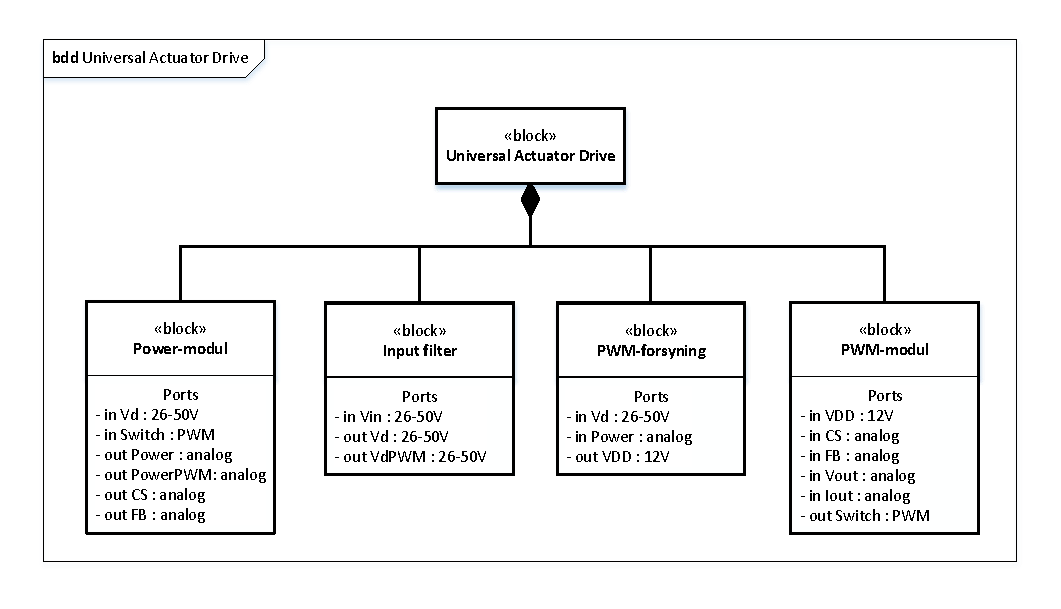
\includegraphics[width=1\linewidth]{../Dokumentation/tex/systemarkitektur/billeder/BDD.pdf}
	\caption{BDD for det overordnede system}
	\label{fig:BDD}
\end{figure}

\noindent Universal Actuator Drive består af fire overordnede blokke - et Power-modul, et Input-filter, en PWM-forsyning og et PWM-modul. Power-modulet indebærer selve effektoverførelsen fra indgang til udgang. Det er i dette modul de dominerende effektafsættelser sker, og derfor også her det termiske design skal optimeres. 

Input-filteret indebærer det filter, der sikrer en stabil indgangsspænding til Power-modulet. Derudover skal det fjerne højfrekvente ripple-spændinger fra indgangssignalet. 

\noindent PWM-forsyningen indebærer en regulator til regulering af PWM-modulets forsyningsspænding. Her vil der udvikles en metode, der forsyner regulatoren fra indgangskilden under opstart, og udgangen når denne er stabil.

PWM-modulet indebærer PWM-controlleren, der skal regulere udgangen til den ønskede belastning. Det sker ved tilpasning af switch-signalet, samt strøm- og spændingsregulering af udgangen.

\section{Internal Block Diagram}
Figur~\ref{fig:IBD} viser et IBD for det samlede system. Det er udarbejdet ud fra systemets BDD. IBD'et giver et overblik over forbindelserne internt i systemet. Det viser også, hvilke forbindelser systemet modtager fra andre systemer. Det vil sige grænsefladerne til omverdenen. Kravene for forbindelserne er nærmere beskrevet i dokumentationenen, afsnit 3.2.

\begin{figure}[H]
	\centering
	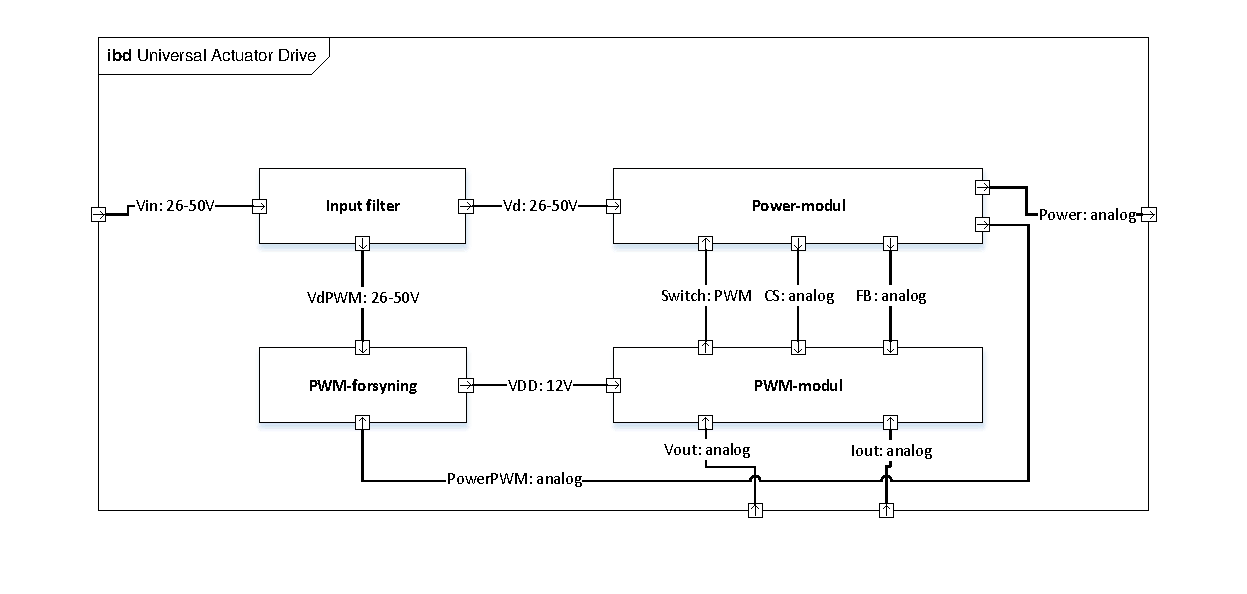
\includegraphics[width=1\linewidth]{../Dokumentation/tex/systemarkitektur/billeder/IBD.pdf}
	\caption{IBD for det overordnede system}
	\label{fig:IBD}
\end{figure}